\chapter{坐标变换}
\section{平移和旋转}
\subsection{坐标轴的平移}\label{subsec:axis_translation}
\noindent
\begin{minipage}{0.58\linewidth}\parindent2em
点的坐标和曲线的方程是对一定的坐标系来说的。
例如,\cref{fig:3-1} 中 $\odot O'$ 的圆心 $O'$,在坐标系 $xOy$ 中的坐标是 $(3,2)$,$\odot O'$ 的方程是 $(x-3)^2+(y-2)^2=5^2$;如果取坐标系 $x'O'y'$($O'x'\parallel Ox,\ O'y'\parallel Oy$),那么在这个坐标系中,它们就分别变成 $(0,0)$ 和 $x^2+y^2=5^2$。

这就是说,对于同一点或者同一曲线,由于选取的坐标系不同,点的坐标或曲线的方程也不同。从上面例子我们看出,把一个坐标系变换为另一个适当的坐标系,可以使曲线的方程简化,便于我们研究曲线的性质。
\end{minipage}\hfill
\begin{minipage}{0.37\linewidth}\centering
\begin{figurehere}
  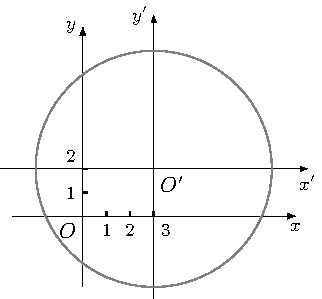
\includegraphics{3-1.pdf}
  \caption{}\label{fig:3-1}
\end{figurehere}
\end{minipage}

\medskip
坐标轴的方向和长度单位都不改变,只改变原点的位置,这种坐标系的变换叫做\Concept{坐标轴的平移}。
简称\Concept{移轴}。

下面研究在平移情况下,同一个点在两个不同的坐标系中坐标之间的关系。


设 $O'$ 在原坐标系 $xOy$ 中的坐标为 $(h,k)$ ,以 $O'$ 为原点平移坐标轴,建立新坐标系 $x'O'y'$。
平面内 任意一点 $M$ 在原坐标系中的坐标为 $(x,y)$,在新坐标系中的坐标为 $(x',y')$,点 $M$ 到 $x$ 轴、$y$ 轴的垂线的垂足分别是 $M_1$、$M_2$。从\cref{fig:3-2} 可以看出,

\noindent
\begin{minipage}{0.62\linewidth}\parindent2em
\begin{align*}
  x&=OO_1+O_1M_1 =h+x', \\
  y&=OO_2+O_2M_2 =k+y'.
\end{align*}
因此,点 $M$ 的原坐标、新坐标之间,有下面的关系:
\begin{equation}
  \label{eq:axis_translation1}
  \tcbhighmath{x=x'+h,\quad y=y'+k}.
\end{equation}
或者写成
\end{minipage}\hfill
\begin{minipage}{0.33\linewidth}\centering
  \begin{figurehere}
    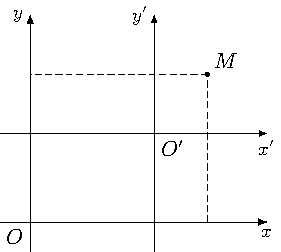
\includegraphics{3-2.pdf}
    \caption{}\label{fig:3-2}
  \end{figurehere}
\end{minipage}
% \medskip\noindent
\begin{equation}
  \label{eq:axis_translation2}
  x'=x-h,\quad y'=y-k.
\end{equation}
\cref{eq:axis_translation1,eq:axis_translation2} 叫做\Concept{平移(移轴)公式}。

\bigskip\noindent
\begin{minipage}{0.62\linewidth}\parindent2em
\begin{example}
  平移坐标轴,把原点移到 $O'\,(3,-4)$(\cref{fig:3-3}),求下列各点的新坐标:$O\,(0,0)$、$A\,(3,-4)$、$B\,(5,2)$、$C\,(3,-2)$。
\end{example}
\begin{solution}
  把已知各点的原坐标分别代入
  \[x'=x-3,\quad y'=y+4,\]
  便得到它们的新坐标:
  \[O\,(-3,4)\quad A\,(0,0)\quad B\,(2,6)\quad C\,(0,2).\]
\end{solution}
\end{minipage}\hfill
\begin{minipage}{0.33\linewidth}
  \begin{figurehere}
    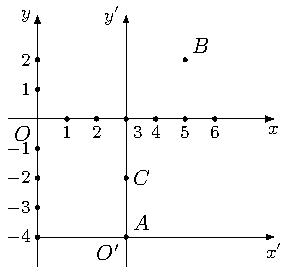
\includegraphics{3-3.pdf}
    \caption{}\label{fig:3-3}
  \end{figurehere}
\end{minipage}

\medskip
\begin{example}
  平移坐标轴,把原点移到 $O'\,(2,-1)$,求下列曲线关于新坐标系的方程,并且画出新坐标轴和曲线:
  \begin{enumerate}
    \item $x=2$;
    \item $y=-1$;
    \item $\dfrac{(x-2)^2}{9}+\dfrac{(y+1)^2}{4}=1$。
  \end{enumerate}
\end{example}
\begin{solution}
  因为坐标系的改变,曲线上每一点的坐标都相应的改变,所以,曲线的方程也要改变。
  设曲线上任意一点的新坐标为 $(x',y')$,那么
  \[x=x'+2,\quad y=y'-1.\]
  
\end{solution}

\noindent
\begin{minipage}{0.6\linewidth}
  代入原方程,就得到新方程:
  \begin{enumerate}
    \item $x'=0$;
    \item $y'=0$;
    \item $\dfrac{x'^2}{9}+\dfrac{y'^2}{4}=1$。
  \end{enumerate}

  \bigskip 新坐标轴和曲线如\cref{fig:3-4}。
\end{minipage}
\begin{minipage}{0.35\linewidth}\centering
\begin{figurehere}
  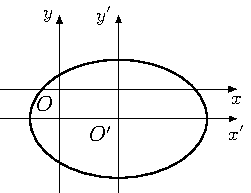
\includegraphics{3-4.pdf}
  \caption{}\label{fig:3-4}
\end{figurehere}
\end{minipage}

\medskip
\begin{Practice}
  \begin{question}
    \item 平移坐标轴,把原点移到 $O'\,(4,5)$。求下列各点的新坐标,并画出新坐标轴和各点:
    \begin{tasks}(4)
      \task $A\,(3,-6)$;
      \task $B\,(7,0)$;
      \task $C\,(-4,5)$;
      \task $D\,(0,-8)$。
    \end{tasks}
    \item 平移坐标轴,把原点移到 $O'\,(2,-3)$。求 $x^2+y^2-4x+6y-3=0$ 在新坐标系中的方程,并画出新坐标轴和图形。
  \end{question}
\end{Practice}

\subsection{利用坐标轴的平移化简二元二次方程}
在\cref{subsec:axis_translation}我们已看到,适当地平移坐标轴可以化简曲线的方程。现在,我们研究如何选择新坐标系来化简方程。
先看下面例子。

\medskip\noindent
\begin{minipage}{0.53\linewidth}\parindent2em
\begin{example}
  平移坐标轴,化简方程
  \[x^2-y^2+8x-14y-133=0,\]
  并画出新坐标系和方程的曲线。
\end{example}
\begin{solution}
  把 $x=x'+h$,$y=y'+k$ 代入方程,得
  \begin{multline*}(x'+h)^2-(y'+k)^2+8(x'+h)\\{}-14(y'+k)-133=0.\end{multline*}
  就是
\end{solution}
\end{minipage}\hfill
\begin{minipage}{0.42\linewidth}\centering
\begin{figurehere}
  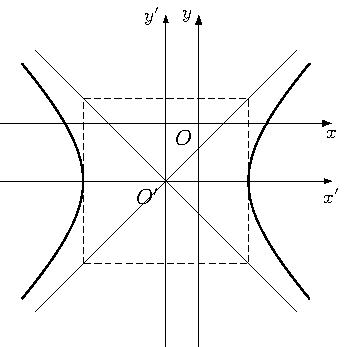
\includegraphics{3-5.pdf}
  \caption{}\label{fig:3-5}
\end{figurehere}
\end{minipage}
\begin{equation}
  \label{eq:translation_expand}
  x'^2-y'^2+(2h+8)x'-(2k+14)y'+h^2-k^2+8h-14k-133=0.
\end{equation}
令
\[2h+8=0,\quad 2k+14=0.\]
解得 $h=-4$,$k=-7$。代入\cref{eq:translation_expand},得
\[x'^2-y'^2=100.\]
这是等轴双曲线。新坐标系和方程的曲线如\cref{fig:3-5}。

\bigskip
上面的例子说明,对于缺 $xy$ 项的二元二次方程
\[ Ax^2+Cy^2+D+E+F=0\quad(A,C\text{不同时为零}),\]
利用坐标轴平移,可以使新方程没有一次项(或没有一个一次项和常数项),从而化成圆锥曲线的标准方程。
但上面的待定系数法,往往不如从原方程配方开始简单。

\begin{example}
  证明二次函数 $y=ax^2+bx+c$($a\neq 0$)的图形是一条抛物线。
\end{example}
\begin{solution}
  把原方程化简,如果能化成抛物线的标准方程,就可以证明它是抛物线。

  因为方程缺 $xy$ 项和 $y^2$ 项,我们将原方程按 $x$ 配方,得
  \[y=a\left(x^2+\frac{b}{a}x+\frac{b^2}{4a^2}\right)+c-\frac{b^2}{4a^2}=a\left(x+\frac{b}{2a}\right)^2+\frac{4ac-b^2}{4a}.\]
  将上式变形为
  \begin{equation}
    \label{eq:parabola_transform}
    \left(x+\frac{b}{2a}\right)^2=\frac{1}{a}\left(y-\frac{4ac-b^2}{4a}\right)
  \end{equation}

  设
  \begin{align*}
    x&=x+\dfrac{b}{2a}, \\
    y&=y-\dfrac{4ac-b^2}{4a},
  \end{align*}
  代入\cref{eq:parabola_transform},得
  \[ x'^2=\frac{1}{a}y'.\]

  因此,二次函数 $y=ax^2+{bx}+c$ 的图形是以 $O'\,\left(-\dfrac{b}{2a},\dfrac{4ac-b^2}{4a}\right)$ 为顶点,对称轴平行于 $y$ 轴的抛物线。当 $a>0$ 时,开口向上;当 $a<0$ 时,开口向下。图形如\cref{fig:3-6}。
\end{solution}
\begin{figure}
  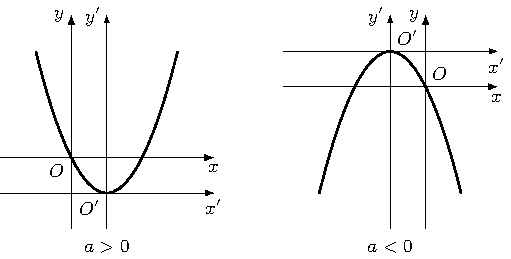
\includegraphics{3-6.pdf}
  \caption{}\label{fig:3-6}
\end{figure}

\bigskip
注意,在初中研究二次函数 $y=ax^2+bx+c$ 的图象时,为使画图方便,我们是先画 $y=ax^2$ 的图象,然后将图象平移,使它的顶点移到 $O'\,\left(-\dfrac{b}{2a},\dfrac{4ac-b^2}{4a}\right)$,得到 $y=ax^2+bx+c$ 的图象。
现在正好相反,在利用坐标法研究图形性质时,为使方程简单,不移动图形,而是把坐标原点移到 $O'\,\left(-\dfrac{b}{2a},\dfrac{4ac-b^2}{4a}\right)$,得到新方程 $y'=ax'^2$,从而容易知道它的性质。

\begin{Practice}
  \begin{question}
    \item 经过怎样的平移变换,可以把方程 $x^2+y^2-6x+12y-4=0$ 化为没有一次项的新方程?
    \item 化简方程 $y=\dfrac{1}{2}x^2+x+\dfrac{5}{2}$,并画出它的图形。
  \end{question}
\end{Practice}
\begin{Exercise}
  \begin{question}
    \item 解答:
    \begin{enumerate}[itemindent=2em]
      \item 平移坐标轴,把原点分别移到何处,点的坐标变化如下:
      \begin{tasks}(2)
        \task $A\,(1,0)\to A\,(4,3)$;
        \task $B\,(2,4)\to B\,(2,-3)$。
      \end{tasks}
      \item 经过坐标轴平移,把原点移到 $O'\,(3,-2)$ 后,$A$、$B$、$C$、$D$ 各点的新坐标分别是 $(0,2)$、$(-3,0)$、$(-1,3)$、$(1,1)$,求它们的原坐标,并画出新坐标轴和各点。
    \end{enumerate}
    \item 平移坐标轴,把原点移到 $O'$,求下列各曲线的新方程,并画出新坐标轴和图形。
    \begin{tasks}(2)
      \task $y=3$,$O'\,(-2,1)$;
      \task $3x-4y=6$,$O'\,(3,0)$;
      \task $x^2+y^2-4x-2y=0$,$O'\,(2,1)$;
      \task $x^2+6x-y+11=0$,$O'\,(-3,2)$ 。
    \end{tasks}
    \item 平移坐标轴化简方程:
    \begin{tasks}(2)
      \task $x^2+y^2+4x+8y-5=0$;
      \task $x^2+2y^2-4x+8y-5=0$;
      \task $4x^2-9y^2+16x-54y-29=0$;
      \task $x^2-4x-y+5=0$。
    \end{tasks}
    \item 求下列各曲线的焦点坐标和对称轴方程:
    \begin{tasks}(2)
      \task $2x^2+y^2-4x-2y=0$;
      \task $x^2-2y^2-6x+4y+3=0$;
      \task $x^2-4x+4y=0$。
    \end{tasks}
    \item 求适合下列条件的曲线方程:
    \begin{tasks}
      \task 中心为 $O'\,(-2,1)$,长半轴长为 10,焦距为 12,焦点在平行于 $x$ 轴的直线上的椭圆;
      \task 虚轴的长是 8,两顶点是 $A\,(2,1)$ 和 $A'\,(2,-5)$ 的双曲线;
      \task 焦点是 $F\,(3,-3)$,准线是 $y=1$ 的抛物线。
    \end{tasks}
  \end{question}
\end{Exercise}

\subsection{坐标轴的旋转}\label{subsec:axis_rotation}
\medskip\noindent
\begin{minipage}{0.55\linewidth}\parindent2em
前面我们学过坐标轴的平移。
现在来讨论坐标轴旋转时,同一点的坐标间的关系。

如果坐标轴的原点和长度单位都不变。
只是坐标轴按同一方向绕原点旋转同一角度,这种坐标系的变换叫做\Concept{坐标轴的旋转},简称\Concept{转轴}。

我们来求转轴时的坐标变换公式。

设坐标轴旋转角为 $\theta$。在平面内任取一点 $M$,它在坐标系 $xOy$ 和 $x'Oy'$ 中的坐标分别为 $(x,y)$ 和 $(x',y')$(\cref{fig:3-7})。
\end{minipage}\hfill
\begin{minipage}{0.4\linewidth}\centering
\begin{figurehere}
  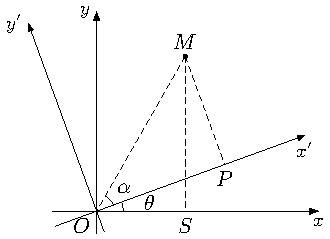
\includegraphics{3-7.pdf}
  \caption{}\label{fig:3-7}
\end{figurehere}
\end{minipage}

\medskip
作 $MS$、$MP$ 分别垂直于 $x$ 轴、$x'$ 轴。连结 $OM$,设 $\angle POM=\alpha$。那么
\begin{align*} 
  x' & = |OM|\cos\alpha, \\
  y' & = |OM|\sin\alpha.
\end{align*}
所以
\begin{align*} 
  x & = |OM|\cos(\theta+\alpha)=|OM|(\cos\theta\cos\alpha-\sin\theta\sin\alpha)\\
    & = x'\cos\theta-y'\sin\theta,\\
  y & = |OM|\sin(\theta+\alpha)=|OM|(\sin\theta\cos\alpha+\cos\theta\sin\alpha)\\
    & = x'\sin\theta+y'\cos\theta.
\end{align*}
也就是
\begin{equation}
  \label{eq:axis_rotation1}
  \tcbhighmath{\begin{aligned}
    x &= x'\cos\theta-y'\sin\theta,\\
    y &= x'\sin\theta+y'\cos\theta.
  \end{aligned}}
\end{equation}

由\cref{eq:axis_rotation1} 解出 $x'$、$y'$,得
\begin{equation}
  \label{eq:axis_rotation2}
  \begin{aligned}
    x' &= x\cos\theta+y\sin\theta,\\
    y' &= -x\sin\theta+y\cos\theta.
  \end{aligned}
\end{equation}

\cref{eq:axis_rotation1} 是用新坐标表示原坐标的旋转变换公式,\cref{eq:axis_rotation2} 是用原坐标表示新坐标的旋转变换公式,统称\Concept{旋转(转轴)公式}。

\cref{eq:axis_rotation2} 还可以用下面方法求出:

如果 $x$ 轴、$y$ 轴旋转 $\theta$ 角到 $x'$ 轴、$y'$ 轴的位置,那么 $x'$ 轴、$y'$ 轴旋转 $-\theta$ 角就到 $x$ 轴、$y$ 轴的位置。
这样,$(x',y')$ 变为点 $M$ 的原坐标,而 $(x,y)$ 就变为它的新坐标。
这时直接把 $-\theta$ 代入\cref{eq:axis_rotation1},得到
\begin{align*}
  x' &= x\cos(-\theta)-y\sin(-\theta),\\
  y' &= x\sin(-\theta)+y\cos(-\theta).
\end{align*}
改写后就是\cref{eq:axis_rotation2}。

\begin{example}
  把坐标轴旋转 $\dfrac{\uppi}{6}$,求点 $P\,(-1,\sqrt{3})$ 在新坐标系中的坐标。
\end{example}
\begin{solution}
  把 $\theta=\dfrac{\uppi}{6}$,$x=-1$,$y=\sqrt{3}$,代入\cref{eq:axis_rotation2},得
  \begin{align*}
    x' &= -1\cdot\cos\dfrac{\uppi}{6}+\sqrt{3}\cdot\sin\dfrac{\uppi}{6}=-\dfrac{\sqrt{3}}{2}+\sqrt{3}\cdot\dfrac{1}{2}=0,\\
    y' &= -(-1)\cdot\sin\dfrac{\uppi}{6}+\sqrt{3}\cdot\cos\dfrac{\uppi}{6}=\dfrac{1}{2}+\sqrt{3}\cdot\dfrac{\sqrt{3}}{2}.
  \end{align*}
  点 $M$ 在新坐标系中的坐标是 $(0,2)$。
\end{solution}

\begin{example}\label{exam:reduction}
  将坐标轴旋转 $\dfrac{\uppi}{3}$,求曲线
  \[2x^2-\sqrt{3}xy+y^2=10\]
  在新坐标系中的方程,并画图。
\end{example}
\begin{minipage}{0.65\linewidth}\parindent2em
\begin{solution}
  把 $\theta=\dfrac{\uppi}{3}$ 代入\cref{eq:axis_rotation1},得
  \begin{align*}
    x &= x'\cos\dfrac{\uppi}{3}-y'\sin\dfrac{\uppi}{3}\theta=\frac{1}{2}x'-\frac{\sqrt{3}}{2}y',\\
    y &= x'\sin\dfrac{\uppi}{3}+y'\cos\dfrac{\uppi}{3}\theta=\frac{\sqrt{3}}{2}x'+\frac{1}{2}y'.
  \end{align*}
  代入方程,得新坐标系的方程
\end{solution}
\end{minipage}\hfill
\begin{minipage}{0.3\linewidth}\centering
\begin{figurehere}
  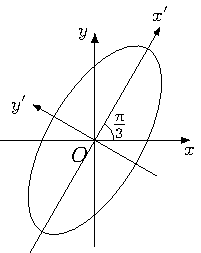
\includegraphics{3-8.pdf}
  \caption{}\label{fig:3-8}
\end{figurehere}
\end{minipage}

\medskip
\[2\left(\frac{1}{2}x'-\frac{\sqrt{3}}{2}y'\right)^2-\sqrt{3}\left(\frac{1}{2}x'-\frac{\sqrt{3}}{2}y'\right)\left(\frac{\sqrt{3}}{2}x'+\frac{1}{2}y'\right)+\left(\frac{\sqrt{3}}{2}x'+\frac{1}{2}y'\right)^2=10
  \]
  化简,得标准方程
  \[ \frac{x'^2}{20}+\frac{y'^2}{4}=1.\]
  它是一个椭圆,画出图形如\cref{fig:3-8}。

\begin{Practice}
  \begin{question}
    \item 设旋转角 $\theta=-\dfrac{\uppi}{4}$,求新坐标系中的两点 $A\,(-3,2)$,$B\,(1,0)$ 在原坐标系的坐标。
    \item 设旋转角 $\theta=\dfrac{\uppi}{6}$,求原坐标系中的两点 $C\,(2,-1)$,$D\,(0,1)$ 在新坐标系的坐标。
    \item 按所给的角 $\theta$ 旋转坐标轴,变换下列各方程:
    \begin{tasks}(2)
      \task $x+y=0$,$\left(\theta=\dfrac{\uppi}{4}\right)$;
      \task $x-y=0$,$\left(\theta=-\dfrac{\uppi}{2}\right)$;
      \task $x^2+y^2=9$,$\left(\theta=\dfrac{\uppi}{3}\right)$;
      \task $x^2-2\sqrt{3}{xy}+3y^2=8$,$\left(\theta=-\dfrac{\uppi}{3}\right)$。
    \end{tasks}
  \end{question}
\end{Practice}

\subsection{利用坐标轴的旋转化简二元二次方程}\label{subsec:axis_rotation_reduction}
从\cref{subsec:axis_rotation}的\cref{exam:reduction} 我们看到,把坐标轴旋转一个适当的角度,可以化简二元二次方程
\begin{equation}
  \label{eq:general_power_2}
  Ax^2+Bxy+Cy^2+Dx+Ey+F=0\quad(B\neq 0)
\end{equation}
使新方程没有 $x'y'$ 项。
如何选择旋转角呢? 下面我们来研究这个问题。

使坐标轴旋转 $\theta$ 角,这时
\begin{align*}
  x &= x'\cos\theta-y'\sin\theta,\\
  y &= x'\sin\theta+y'\cos\theta.
\end{align*}
代入\cref{eq:general_power_2},可得
\begin{equation}
  \label{eq:general_power_2_rotated}
  A'x'^2+B'x'y'+C'y'^2+D'x'+E'y'+F'=0,
\end{equation}
这里,
\begin{align*}
  A' &= A\cos^2\theta+B\sin\theta\cos\theta+C\sin^2\theta,\\
  B' &= -2A\sin\theta\cos\theta+B\cos^2\theta-B\sin^2\theta+2C\sin\theta\cos\theta,\\
  C' &= A\sin^2\theta-B\sin\theta\cos\theta+C\cos^2\theta,\\
  D' &= D\cos\theta+E\sin\theta,\\
  E' &= -D\sin\theta+E\cos\theta.
\end{align*}
为了使 $B'=0$,即
\[ -2A\sin\theta\cos\theta+ B(\cos^2\theta-\sin^2\theta)+2C\sin\theta\cos\theta=0,\]
也就是使
\[ B\cos {2\theta } = \left( {A - C}\right) \sin {2\theta }\]
只要取 $\theta$ 满足下式就可以了:
\begin{equation}
  \label{eq:rotation_angle}
\tcbhighmath{\cot2\theta=\frac{A-C}{B}}.
\end{equation}

取满足\cref{eq:rotation_angle} 的角 $\theta$,作旋转变换,就可以使\cref{eq:general_power_2_rotated} 中没有 $x'y'$ 项。

由于旋转公式里只用到 $\sin\theta$ 和 $\cos\theta$ 的值,因此不一定要求出 $\theta$ 角的度数,有时可直接利用下列三角恒等式来计算 $\sin\theta$、$\cos\theta$。
\begin{equation}
  \label{eq:theta_trigono_function}
  \begin{cases}
    \cos2\theta=\dfrac{\cot2\theta}{\sqrt{1+\cot^22\theta}},\\[15pt]
    \sin\theta=\sqrt{\dfrac{1-\cos2\theta}{2}},\\[10pt]
    \cos\theta=\sqrt{\dfrac{1+\cos2\theta}{2}}.
  \end{cases}
\end{equation}

要使新方程不含 $x'y'$ 项,只要取 $2\theta$ 的最小正值即可,也就是取 $0<2\theta< \uppi$,$0<\theta<\frac{\uppi}{2}$,这时 $\cos2\theta$ 和 $\cot2\theta$ 的符号相同,$\sin\theta$ 和 $\cos\theta$ 都是正值,因此,\cref{eq:theta_trigono_function} 根号前都取正号。

例如\cref{subsec:axis_rotation}的\cref{exam:reduction},对于方程 $2x^2-\sqrt{3}xy+y^2=10$,如果事先不给出 $\theta$,而要把它化简,我们可利用\cref{eq:rotation_angle} 求出
\[\cot2\theta=\frac{2-1}{-\sqrt{3}}=-\frac{1}{\sqrt{3}}\]
代入\cref{eq:theta_trigono_function},得
\begin{align*}
  \cos2\theta&=\dfrac{-\dfrac{1}{\sqrt{3}}}{\sqrt{1+\dfrac{1}{3}}}=-\frac{1}{2},\\[8pt]
  \sin\theta&=\sqrt{\dfrac{1-\dfrac{1}{2}}{2}}=\frac{\sqrt{3}}{2},\\[8pt]
  \cos\theta&=\sqrt{\dfrac{1+\dfrac{1}{2}}{2}}=\frac{1}{2}.
\end{align*}
这样就可直接写出旋转公式
\begin{align*}
  x&=\frac{1}{2}x'-\frac{\sqrt{3}}{2}y',\\
  y&=\frac{\sqrt{3}}{2}x'+\frac{1}{2}y'.
\end{align*}

\begin{example}
  利用坐标轴的旋转化简方程:
  \[2x^2+4xy+5y^2-22=0\]
  并画出它的图形。
\end{example}
\noindent
\begin{minipage}{0.65\linewidth}\parindent2em
\begin{solution}
  \begin{align*}
    \cot2\theta&=\dfrac{2-5}{4}=-\frac{3}{4},&
    \cos2\theta&=\dfrac{-\dfrac{3}{4}}{\sqrt{1+\dfrac{9}{16}}}=-\frac{3}{5}.\\
    \sin \theta&=\sqrt{\frac{1+\dfrac{3}{5}}{2}}=\frac{2}{\sqrt{5}},&
    \cos \theta&=\sqrt{\frac{1-\dfrac{3}{5}}{2}}=\frac{1}{\sqrt{5}}.
  \end{align*}
\end{solution}
\end{minipage}\hfill
\begin{minipage}{0.3\linewidth}\centering
\begin{figurehere}
  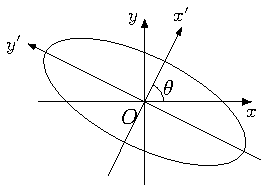
\includegraphics{3-9.pdf}
  \caption{}\label{fig:3-9}
\end{figurehere}
\end{minipage}

\bigskip\noindent
因此旋转公式是
  \[ x=\frac{x'-2y'}{\sqrt{5}},\quad y=\frac{2x'+y'}{\sqrt{5}}.\]
  代入原方程,得
  \begin{gather*}
    2\left(\frac{x'-2y'}{\sqrt{5}}\right)^2+4\left(\frac{x'-2y'}{\sqrt{5}}\right)\left(\frac{2x'+y'}{\sqrt{5}}\right)+5\left(\frac{2x'+y'}{\sqrt{5}}\right)^2-22=0.\\
    6x'^2+y'^2=22,
  \end{gather*}
即
  \[\frac{x'^2}{\dfrac{11}{3}}+\frac{y'^2}{22}=1.\]

  根据 $\sin\theta=\dfrac{2}{\sqrt{5}}$,得旋转角 $\theta \approx \ang{63;26;}$。方程表示的曲线是长轴长是 $2\sqrt{22}$,短轴长是 $\dfrac{2}{3}\sqrt{33}$ 的椭圆。画出图形,如\cref{fig:3-9}。

\begin{example}
  利用坐标轴的旋转,化简方程
  \[x^2+2xy+y^2-2\sqrt{2}x+2\sqrt{2}y=0,\]
  使它不含 $x'y'$ 项。
\end{example}
\begin{solution}
\begin{gather*}
  \cot 2\theta=\frac{1-1}{2}=0,\\ 
  2\theta=\frac{\uppi}{2},\quad \theta=\frac{\uppi}{4}.
\end{gather*}
因此旋转公式是
\begin{align*}
  x&=\dfrac{\sqrt{2}}{2}(x'-y'),\\
  y&=\dfrac{\sqrt{2}}{2}(x'+y').
\end{align*}
代入原方程,得
\begin{multline*}
  \left[\dfrac{\sqrt{2}}{2}(x'-y')\right]^2+2\left[\dfrac{\sqrt{2}}{2}(x'-y')\right]\left[\dfrac{\sqrt{2}}{2}(x'+y')\right]+\left[\dfrac{\sqrt{2}}{2}(x'+y')\right]^2\\
  -2\sqrt{2}\left[\dfrac{\sqrt{2}}{2}(x'-y')\right]+2\sqrt{2}\left[\dfrac{\sqrt{2}}{2}(x'+y')\right]=0
\end{multline*}
整理后,得
\[x'^2+2y'^2=0.\]
\end{solution}

\begin{Practice}
  化简下列方程,并画图形:
  \begin{tasks}
    \task $x^2-2xy+y^2=12$;
    \task $4x^2+8xy-2y^2-7=0$。
  \end{tasks}
\end{Practice}

\begin{Exercise}
  \begin{question}
    \item 把点 $A\,(4,3)$ 的坐标变成 $\,(3,4)$,坐标轴应旋转多大角度?
    \item 坐标轴旋转多大角度,才能使点 $M\,(1,2+\sqrt{3})$ 的横、纵坐标相等? 求出点 $M$ 的新坐标。
    \item 将坐标轴旋转 $\frac{\uppi}{3}$ 后,点 $M$ 的坐标变为 $(1,2)$。求点 $M$ 在原坐标系的坐标。
    \item 将坐标轴旋转 $-\frac{\uppi}{2}$,求椭圆 $x^2+\frac{y^2}{2}=1$ 在新坐标系中的方程。
    \item 将坐标轴旋转 $\frac{\uppi}{2}$,求抛物线 $y^2=2px$ 在新坐标系中的方程。
    \item 证明:不论坐标轴旋转多大角度,方程 $x^2+y^2=r^2$ 的形式不变。
    \item 利用坐标轴旋转,化简下列方程,并画出图形:
    \begin{tasks}
      \task $x^2+4xy+y^2=16$;
      \task $21x^2-10\sqrt{3}xy+31y^2=144$。
    \end{tasks}
  \end{question}
\end{Exercise}

\section{一般二元二次方程的讨论}
\subsection{化一般二元二次方程为标准式}
我们已经知道,坐标轴旋转适当的角度,可以化简二元二次方程
\[Ax^2+Bxy+Cy^2+Dx+Ey+F=0\quad(A,B,C\text{ 不全为零}),\]
使新方程中没有 $x'y'$ 项。对于不含 $x'y'$ 项的二次方程,通过平移还可以继续化简,在一般情况下,最后能够化成圆锥曲线的标准方程。
\begin{example}
  把方程
  \[x^2+2xy+y^2+3x+y=0\]
  化成圆锥曲线的标准方程,并画出图形。
\end{example}
\begin{solution}
  \begin{gather*}
    \because\quad \cot2\theta=\frac{1-1}{2}=0,\\
    2\theta=\frac{\uppi}{2},\quad\theta=\frac{\uppi}{4}.\\
    \therefore\quad \sin\theta=\frac{\sqrt{2}}{2},\ \cos\theta=\frac{\sqrt{2}}{2}
  \end{gather*}
  因此
  \begin{align*}
    x&=\dfrac{\sqrt{2}}{2}(x'-y'),\\
    y&=\dfrac{\sqrt{2}}{2}(x'+y').
  \end{align*}
  代入原方程,化简得
  \[2x'^2+2\sqrt{2}x'-\sqrt{2}y'=0\]
\end{solution}

\noindent
\begin{minipage}{0.6\linewidth}%\parindent2em
  配方,得
  \[2\left(x'+\dfrac{\sqrt{2}}{2}\right)^2=\sqrt{2}\left(y'+\dfrac{\sqrt{2}}{2}\right)\]
  再作平移变换,设
  % \begin{align*}
  \[
    x''=x'+\dfrac{\sqrt{2}}{2},\quad
    y''=y'+\dfrac{\sqrt{2}}{2}.
  % \end{align*}
  \]
\end{minipage}\hfill
\begin{minipage}{0.32\linewidth}\centering
\begin{figurehere}
  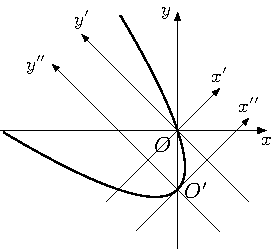
\includegraphics{3-10.pdf}
  \caption{}\label{fig:3-10}
\end{figurehere}
\end{minipage}

\medskip\noindent
代入上式得 $2x''^2= \sqrt{2}y''$,即
\[x''^2= \frac{\sqrt{2}}{2}y''.\]
由此可知,原方程的图形是抛物线,画出图形如\cref{fig:3-10}。

\begin{example}\label{exam:parallel_lines}
  证明:二元二次方程 $x^2+2xy+y^2+2x+2y-3=0$ 表示两条平行直线。
\end{example}
\begin{proof}
  化简方程。因为 $B\neq 0$,所以先转轴。
  \begin{gather*}
    \cot 2\theta=\frac{1-1}{2}=0,\\
    \theta=\frac{\uppi}{4}.
  \end{gather*}
  因此旋转公式是
  \[ x=\frac{\sqrt{2}}{2}(x'-y'),\quad y=\frac{\sqrt{2}}{2}(x'+y')\]
  代入原方程,得
  \[ 2x'^2+2\sqrt{2}x'-3=0.\]
  配方,得
  \begin{gather*}
    2\left(x+\frac{\sqrt{2}}{2}\right)^2=4,\\
    \left(x+\frac{\sqrt{2}}{2}\right)^2=2.
  \end{gather*}
  即
  \begin{gather*}
    x'+\frac{\sqrt{2}}{2}=\sqrt{2},\quad x'+\frac{\sqrt{2}}{2}=-\sqrt{2}.\\
    x'=\frac{\sqrt{2}}{2},\quad x'=-\frac{3\sqrt{2}}{2}.
  \end{gather*}
  这是平行于 $y'$ 轴的两条平行直线。所以方程
  \[x^2+2xy+y^2+2x+2y-3=0\]
  表示两条平行直线。
\end{proof}

\cref{exam:parallel_lines} 还可以用下面方法证明。

把方程左边因式分解,得
\begin{gather*}
  (x+y)^2+2(x+y)-3=0,\\
  (x+y+3)(x+y-1)=0,
\end{gather*}
得
\[ x+y+3=0,\quad x+y-1=0.\]
因为它们的斜率相等,但截距不同,所以方程表示两条平行直线。

\begin{Practice}
  \begin{question}
    \item 化简方程 $3x^2-10xy+3y^2+26x-22y+35=0$。
    \item 化简方程 $4xy-3x^2+4=0$,画出它的图形。
  \end{question}
\end{Practice}

\subsection{一般二元二次方程的讨论}
我们知道,一般二元二次方程,经过坐标轴的旋转和平移,可以化成圆锥曲线的标准方程,从而知道它所表示的曲线的形状和位置。
但是,化简过程常常是很繁的。
现在,我们研究一下化简前后方程的系数之间的关系,找出直接由方程的系数判别方程类型的方法。

设二元二次方程
\begin{equation}
  \label{eq:power2_curve_general_equation}
  Ax^2+Bxy+Cy^2+Dx+Ey+F=0
\end{equation}
是某曲线的方程,这里 $A$、$B$、$C$ 不全为零。

首先,我们把坐标轴旋转 $\theta$ 角,使新方程没有 $x'y'$ 项。这时\cref{eq:power2_curve_general_equation} 变成
\begin{equation}
  \label{eq:power2_curve_transform}
  A'x'^2+C'y'^2+D'x+E'y+F'=0
\end{equation}
由\cref{subsec:axis_rotation_reduction}知道,其中
\begin{gather}
  \label{eq:transform3} A\cos^2\theta+B\sin\theta\cos\theta+C\sin^2\theta=A',\\
  \label{eq:transform4} -(A-C)\sin2\theta+B\cos2\theta=0,\\
  \label{eq:transform5} A\sin^2\theta-B\sin\theta\cos\theta+C\cos^2\theta=C'.
\end{gather}
把\cref{eq:transform3,eq:transform5} 的两边相加,得
\begin{equation}
  \label{eq:transform6}
  A+C=A'+C',
\end{equation}
\cref{eq:transform3,eq:transform5} 的两边相减,得
\begin{equation}
  \label{eq:transform7}
  (A-C)\cos2\theta+B\sin2\theta=A'-C',
\end{equation}
\cref{eq:transform4,eq:transform7} 两边平方后相加,得
\begin{equation}
  \label{eq:transform8}
  (A-C)^2+B^2=(A'-C')^2.
\end{equation}
从\cref{eq:transform8} 的两边减去\cref{eq:transform6} 的两边的平方,得
\[B^2-4AC=-4A'C'.\]

这就是坐标变换前后方程的二次项系数之间的关系。下面我们研究如何利用这个关系式判别方程的类型。
\begin{enumerate}[1.]
  \item 如果 $B^2-4AC\neq 0$,那么 $A'C'\neq 0$,即 $A'$、$C'$ 都不等于零。这时,把\cref{eq:power2_curve_transform} 配方,得
  \[A'(x'-h)^2+C'(y'-k)^2=F',\]
  经过平移变换,方程可写成下面形式:
  \[A'x''^2+C'y''^2=F'.\]
  \begin{enumerate}
    \item 如果 $B^2-4AC<0$,那么 $A'C'>0$ ,所以 $A'$、$C'$ 符号相同,方程的曲线是椭圆($A'$、$C'$ 的符号和 $F'$ 相同时)、或者是一个点($F'=0$ 时)、或者没有轨迹 ($A'$、$C'$ 的符号和 $F'$ 相反时)。我们把 $B^2-4AC<0$ 时的二元二次方程叫做\Concept{椭圆型方程}。
    \item 如果 $B^2-4AC>0$,那 $A'C'<0$ ,所以 $A'$、$C'$ 的符号相反,方程的曲线是双曲线($F'\neq 0$ 时)、或者两条相交直线($F'=0$ 时)。我们把 $B^2-4AC>0$ 时的二元二次方程叫做\Concept{双曲线型方程}。
  \end{enumerate}
  \item 如果 $B^2-4AC=0$,那么 $A'C'=0$。
  
  由转轴过程我们看到,经过变换,方程的次数并不改变,\cref{eq:power2_curve_transform} 仍是二次方程,所以 $A'$、$C'$ 不能同时为零。
  \begin{enumerate}
    \item\label{itm:step1} 当 $A'= 0$,$C'\neq 0$ 时,\cref{eq:power2_curve_transform} 变为
    \[C'y'^2+D'x'+E'y'+F=0.\]

    如果 $D'\neq 0$,把上式配方,可变为下面形式:
    \[C'(y'-k')^2+D'(x'-h')=0.\]
    再经过平移变换,得
    \[C'y''^2=-D'x'',\]
    这是一条抛物线;

    如果 $D'=0$,\cref{eq:power2_curve_transform} 变成下面的形式:
    \[C'y'^2+E'y'+F=0,\]
    这是两条平行直线(方程有两个不相同的实数解时)、或者两条重合直线(方程有两个相同的实数解时)、或者没有轨迹(方程没有实数解时)。
    \item 当 $A'\neq 0$,$C'=0$ 时,讨论同 \ref{itm:step1} 相仿。
  \end{enumerate}

  我们把 $B^2-4AC=0$ 时的二元二次方程叫做\Concept{抛物线型方程}。
\end{enumerate}

$B^2-{4AC}$ 叫做一般二元二次方程的判别式。根据判别式,不需要化简方程,就能够判别一般二元二次方程的类型:
\begin{table}
  \begin{tblr}{colspec={cccX[c]},hline{3}={0.8pt}}
    \SetCell[c=4]{m,c}{方程 $Ax^2+Bxy+Cy^2+Dx+Ey+F=0$}&&&\\
    判别式&类型&一般情形&特殊情形(退缩圆锥曲线)\\
    $B^2-4AC<0$ & 椭圆型   & 椭圆或圆 & 一点或没有轨迹\\
    $B^2-4AC>0$ & 双曲线型 & 双曲线   & 两条相交直线\\
    $B^2-4AC=0$ & 抛物线型 & 抛物线   & 两条平行直线,两条重合直线或没有轨迹\\
  \end{tblr}
\end{table}

对于方程 $A'x''^2+C'y''^2=F'$ ,用 $-x''$ 代 $x''$ ,同时用 $-y''$ 代 $y''$ ,方程不变,所以椭圆型和双曲线型方程的曲线是有一个对称中心的中心对称图形,这样的曲线统称\Concept{有心曲线}。抛物线型方程的曲线没有对称中心(特殊情况下没有确定的对称中心),这样的曲线统称\Concept{无心曲线}。

化简有心曲线的方程时,也可以先移轴,将坐标原点移到曲线的对称中心再转轴;而对于无心曲线,由于无法确定新坐标的原点,所以化简方程时要先转轴后移轴。

\begin{example}
  判别下列方程的类型:
  \begin{enumerate}
    \item $5x^2+12xy-22y^2-12y-19=0$;
    \item $x^2+2xy+y^2+3x+y=0$。
  \end{enumerate}
\end{example}
\begin{solution}
  \begin{enumerate}
    \item $\because\quad B^2-4AC=12^2+4\times5\times22>0$,
    
    $\therefore\quad$ 方程是双曲线型。
    \item $\because\quad B^2-4AC=2^2-4=0$,
    
    $\therefore\quad$ 方程是抛物线型。
  \end{enumerate}
\end{solution}

\begin{example}
  化简方程
  \[2x^2+4xy+5y^2+4x+16y+14=0.\]
\end{example}
\begin{solution}
  因为 $B^2-4AC<0$,所以方程是椭圆型,化简方程时可以先移轴后转轴。

  先移轴。把 $x=x'+h$,$y =y'+k$ 代入方程,得
  \[2(x'+h)^2+ 4(x'+h)(y'+k)+5(y'+k)^2+4(x'+h)+16(y'+k)+14=0,\]
  \begin{multline*}
    2x'^2+4x'y'+5y'^2+(4h+4k+4)x'+(4h+10k+16)y'\\ {}+2h^2+4hk+5k^2+4h+16k+14=0.
  \end{multline*}
  令一次项系数等于零,得
  \[\begin{cases}
    4h+4k+4=0,\\4h+10k+16=0.
  \end{cases}\]
  解方程组,得 $h=1$,$k=-2$。把原点移到 $O'\,(1,-2)$,得新方程
  \[ 2x'^2+4x'y'+5y'^2=0.\]

  再转轴。
  \begin{gather*}
    \cot2\theta=\frac{2-5}{4}= -\frac{3}{4},\\
    \cos2\theta=\frac{-\dfrac{3}{4}}{\sqrt{1+\left(-\dfrac{3}{4}\right)^2}}=-\frac{3}{5},\\
    \sin\theta=\frac{2}{\sqrt{5}},\quad\cos\theta=\frac{1}{\sqrt{5}}.
  \end{gather*}
  旋转公式是
  \begin{align*}
    x'&=\frac{1}{\sqrt{5}}(x''-2y''),\\
    y'&=\frac{1}{\sqrt{5}}(2x''+y'').
  \end{align*}
  代入新方程,化简后得
  \[ 6x''^2+y''^2=0.\]
  适合这个方程的 $x''$ 和 $y''$ 的值只有下面一个解:
  \[\begin{cases}x''=0,\\y''=0.\end{cases}\]

  所以这个方程的图形是一个点,就是移轴后的坐标原点 $O'$。对于原坐标系来说,方程的图形是点 $O'\,(1,-2)$。
\end{solution}

\begin{Practice}
  判别下列方程的类型:
  \begin{question}
    \item $3x^2-7xy+5y^2+x-3y-3=0$;
    \item $5x^2+12xy+5y^2-18x-18y+9=0$;
    \item $2x^2+2xy+y^2+2x+2y-4=0$;
    \item $x^2+2xy+y^2+2x+2y-4=0$。
  \end{question}
\end{Practice}

\begin{Exercise}
  \begin{question}
    \item 化下列方程为标准形式,并画出图形:
    \begin{tasks}
      \task $5x^2+6xy+5y^2+22x-6y+21=0$;
      \task $9x^2-24xy+16y^2-20x-140y+200=0$。
    \end{tasks}
    \item 化简方程 $x^2-2xy+y^2=12$,并画出图形。
    \item 求双曲线 $xy=32$ 的顶点坐标。
    \item 判别下列二次方程的类型:
    \begin{tasks}
      \task $x^2-y^2-4x-2y+1=0$;
      \task $5x^2+y^2-2x+3y-1=0$;
      \task $9x^2-6x-4y+29=0$;
      \task $2x^2+5xy+2y^2-6x-3y+5=0$;
      \task $9x^2-30xy+25y^2+8x-15y=0$。
    \end{tasks}
    \item 方程 $2x^2+\lambda xy+4y^2-7x+\lambda^2y+3=0$ 中,$\lambda$ 取什么值时,方程是:
    \begin{tasks}(3)
      \task 椭圆型;
      \task 双曲线型;
      \task 抛物线型?
    \end{tasks}
    \item 判断下列方程有没有中心,如果有,求出中心坐标:
    \begin{tasks}
      \task $5x^2-26xy+5y^2-16x-16y-52=0$;
      \task $x^2+4xy+4y^2+2x-y+3=0$;
      \task $4xy-4(x+y)+3=0$;
      \task $x^2+2xy+y^2+2x+2y-3=0$。
    \end{tasks}
  \end{question}
\end{Exercise}
\section*{小结}
\begin{enumerate}[C、,itemindent=4.5em]
  \item 坐标变换是解析几何的一种重要工具。
  在本章里,介绍了直角坐标系的坐标轴平移变换,给出了变换公式,并研究了利用移轴化简缺 $xy$ 项的二元二次方程。
  作为选学内容,介绍了坐标轴旋转变换,利用移轴和转轴化简一般二元二次方程,并通过对一般二元二次方程的讨论,总结出利用判别式 $B^2-4AC$ 判别方程类型的一种方法。
  \item 在坐标变换下,点的坐标或曲线的方程一般都发生了变化,但点或曲线本身并不变,即曲线的形状和大小与坐标系的选择无关;另一方面,经过移轴和转轴,方程的次数没有变,并且经过适当的转轴,可使变换前后二元二次方程的二次项系数之间满足等式 $B^2- 4AC=-4A'C'$。因此,我们可以利用坐标变换化简方程,研究曲线,也可以通过判别式,直接判别一般二次曲线的类型。
  
  对于每个二元二次方程,都可以用先转轴后移轴的方法化简,但学过一般二元二次方程类型的判别式后,可以先判别方程的类型,对有心曲线也可以用先移轴后转轴的方法化简,这样有时比较简单。
  \item 一般的二元二次方程 $Ax^2+Bxy+Cy^2+Dx+Ey+F=0$($A$、$B$、$C$ 不全为零)的图形是圆锥曲线(包括退缩圆锥曲线)。用不为零的系数,例如 $A$,除方程的两边后,得
  \[x^2+\frac{B}{A}xy+\frac{C}{A}y^2+\frac{D}{A}x+\frac{E}{A}y+\frac{F}{A}=0.\]
  这就是说,圆锥曲线的方程中,有五个系数是独立的,因此,确定圆锥曲线一般要有五个独立条件。

  当 $B=0$,$A=C$ 时,方程变成
  \[x^2+y^2+\frac{D}{A}x+\frac{E}{A}y+\frac{F}{A}=0,\]
  在一般情况下它表示一个圆。
  因此确定一个圆的方程只要三个独立条件就够了。
\end{enumerate}
\chapter*{复习参考题\chinese{chapter}}
\section*{A 组}
\begin{question}
  \item 平移坐标轴,把原点移到 $O'\,(-4,2)$,求下列各点的新坐标,并画出新坐标轴和各点:
  \[A\,(-8,3);\quad B\,(2,3);\quad C\,(-4,2);\quad O\,(0,0)\]
  \item 平移坐标轴后,原点移到 $O'\,(1,-2)$,$A$、$B$、$C$、$D$ 各点的新坐标分别是 $(-1,1)$、$(0,-2)$、$(3,2)$、$(2,0)$,求它们的原坐标,并画出原坐标轴和各点。
  \item 经过坐标轴平移后,点 $A$ 的坐标由 $(2,-1)$ 变为 $\,(-2,1)$。求坐标原点在新坐标系中的坐标。
  \item 利用坐标变换化简下列各方程,并画出图形:
  \begin{tasks}(2)
    \task $2x^2-y^2+6x+2y+3=0$;
    \task $y^2-4y-4x+16=0$;
    \task $x^2+4y^2+8x-16y=17$;
    \task $x^2+y^2-4x-2y=0$;
    \task $\dfrac{3}{4}x^2-\dfrac{\sqrt{3}}{2}{xy}+\dfrac{1}{4}y^2-\dfrac{9}{2}x-\dfrac{\sqrt{3}}{2}y=0$;
    \task $x^2+12xy+y^2 -4\sqrt{2}x+4\sqrt{2}y=0$ 。
  \end{tasks}
  \item 已知椭圆的两轴平行于坐标轴,长、短半轴长分别是 $a$ 和 $b$,中心在 $C\,(x_0,y_0)$。写出它的方程。
  \item 已知双曲线的中心在 $A\,(x_0,y_0)$,焦距是 $2c$,实轴长是 $2a$,平行于 $y$ 轴。求它的方程。
  \item 已知抛物线的焦点在 $F\,(a,b)$,焦点到准线的距离是 $p$,抛物线的轴平行于 $y$ 轴,求它的方程。
  \item 如果坐标原点不动,把坐标轴旋转怎样的角,才能使点 $A\,(-2,3)$ 落在新坐标系的纵坐标轴上?
  \item 证明:任何二元一次方程都可以用移轴和转轴把它化为 $x''= 0$。
  \item 证明:经过坐标轴的平移和旋转,两点距离公式不变。
  \item 说明下列坐标变换,是怎样的变换:
  \begin{tasks}(3)
    \task  $\begin{cases} x=x'-5,\\y=y'+4; \end{cases}$
    \task* $\begin{cases} x=-\dfrac{\sqrt{3}}{2}x'-\dfrac{1}{2}y',\\y=\dfrac{1}{2}x'-\dfrac{\sqrt{3}}{2}y'; \end{cases}$
    \task  $\begin{cases} x=y',\\y=-x'; \end{cases}$
    \task* $\begin{cases} x=\dfrac{\sqrt{2}}{2}x''-\dfrac{\sqrt{2}}{2}y''+2,\\y=\dfrac{\sqrt{2}}{2}x''+\dfrac{\sqrt{2}}{2}y''-3. \end{cases}$
  \end{tasks}
  \item 判别方程
  \[(1-e^2)x^2+y^2-2epx+e^2p^2=0\]
  当 
  \begin{tasks}(3)
    \task $e=\dfrac{\sqrt{3}}{2}$;
    \task $e=\dfrac{1}{2}$;
    \task $e=1$。
  \end{tasks}
  时各表示什么类型的曲线?
\end{question}
\section*{B 组}
\begin{question}[resume]
  \item 将下列方程化为标准方程,并求焦点坐标及准线方程:
  \begin{tasks}
    \task $4x^2+9y^2+16x-72y+124=0$;
    \task $x^2-y^2+8x-2y+16=0$;
    \task $y^2-10y-4x+21=0$。
  \end{tasks}
  \item 将下列方程化为标准方程,并求焦点坐标及准线方程:
  \begin{tasks}
    \task $3x^2-4xy-4=0$;
    \task $4x^2+4xy+y^2+6x-12y=0$;
    \task $29x^2-24xy+36y^2+82x-96y-91=0$。
  \end{tasks}
  \item 讨论方程 $y=\dfrac{ax+b}{cx+d}$ 的轨迹,并画出图形。
  \begin{tasks}
    \task 当 $c=0$,$d\neq0$ 时;
    \task 当 $c\neq 0$,$bc\neq ad$ 时。
  \end{tasks}
  \item 已知椭圆的两焦点是 $F_1\,(-2,\dfrac{3}{2})$、$F_2\,(2,-\dfrac{3}{2})$,离心率 $e=\dfrac{\sqrt{2}}{2}$,求这个椭圆的方程。
  \item 已知双曲线的两个焦点是 $F_1\,(4,-4)$、$F_2\,(-2,2)$,两条渐近线互相垂直。求双曲线的方程。
\end{question}